\documentclass[11pt,onecolumn,lineno]{olplainarticle}
% Use the lineno option to display guide line numbers if required.

\usepackage[utf8]{inputenc}
\usepackage{graphicx}
\usepackage{hyperref}
\usepackage{lineno}
\linenumbers


\begin{document}

\section*{Supporting Information}

%% Authors should submit SI as a single separate PDF file, combining
%% all text, figures, tables, movie legends, and SI references.  PNAS
%% will publish SI uncomposed, as the authors have provided it.
%% Additional details can be found here:
%% \href{http://www.pnas.org/page/authors/journal-policies}{policy on
%% SI}.  For SI formatting instructions click
%% \href{https://www.pnascentral.org/cgi-bin/main.plex?form_type=display_auth_si_instructions}{here}.
%% The PNAS Overleaf SI template can be found
%% \href{https://www.overleaf.com/latex/templates/pnas-template-for-supplementary-information/wqfsfqwyjtsd}{here}.
%% Refer to the SI Appendix in the manuscript at an appropriate point
%% in the text. Number supporting figures and tables starting with S1,
%% S2, etc.

%% Authors who place detailed materials and methods in an SI Appendix
%% must provide sufficient detail in the main text methods to enable a
%% reader to follow the logic of the procedures and results and also
%% must reference the SI methods. If a paper is fundamentally a study
%% of a new method or technique, then the methods must be described
%% completely in the main text.

\setcounter{figure}{0}
\setcounter{table}{0}

\subsection*{Median Lichen Thallus Area}

To determine the cell size for the grids used to quantify the lichen
occurrences, we quantified the thallus size of the largest and most
abundant species, \textit{Xanthomendoza galericulata}. On each of 73
trees a total of 10 thalli of \textit{X. galericulata} were randomly
selected. The area of each thallus was measured using the length of
across the largest possible measurement from the margin of one-side to
the opposite margin and the length of a line perpendicular to that
from margin to margin. These two measurements were then used to
calculate the area of an ellipse (Area = $\pi (l_1 \dot l_2)$), which
was used to approximate the area of the thallus. The median thallus
size was then calculated from the 10 area measurements for each
tree. The median lichen thallus area of the was less than 0.1 cm$^2$,
and rarely did the median thallus area exceed 0.5 cm$^2$
(Fig.~\ref{fig:SI_xg_median}).

\begin{figure}[ht]
\centering
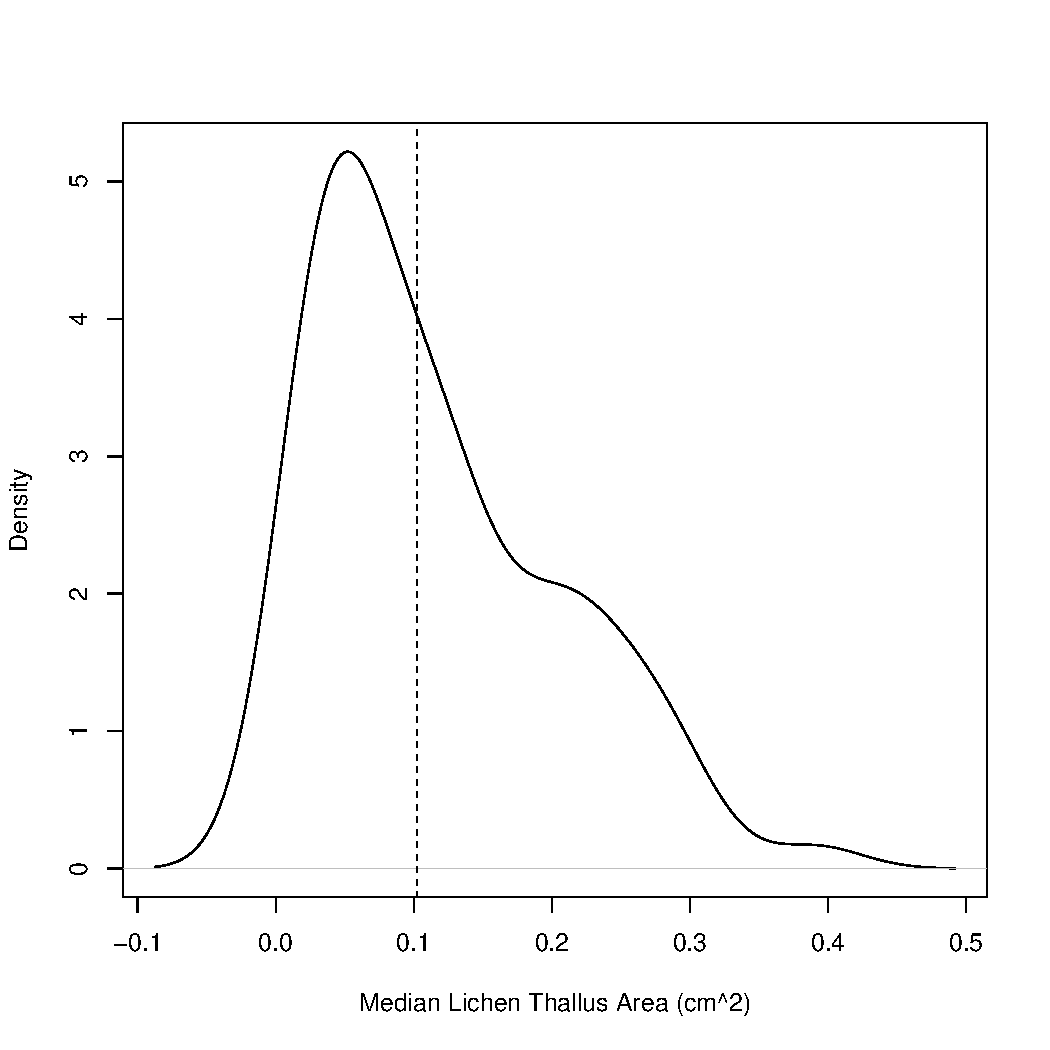
\includegraphics[width=\linewidth]{figures/xg_size.pdf}
\caption{Density plot of the median lichen thallus area (cm$^2$). }
\label{fig:SI_xg_median}
\end{figure}

%% \subsection{Lichen Community Composition Did Not Respond to Genotype}

%% <<<<<<< HEAD
% latex table generated in R 4.0.2 by xtable 1.8-4 package
% Sat Aug 22 17:10:18 2020
=======
% latex table generated in R 3.6.3 by xtable 1.8-4 package
% Wed Oct 14 17:29:46 2020
>>>>>>> 888db0f1e8299aba6255798d27ff3a15e4834c05
\begin{table}[ht]
\centering
\begin{tabular}{lrrrrr}
  \hline
 & Df & SumOfSqs & R2 & F & Pr($>$F) \\ 
  \hline
geno & 9.0000 & 1.5049 & 0.2001 & 0.7507 & 0.8878 \\ 
  Residual & 27.0000 & 6.0143 & 0.7999 &  &  \\ 
  Total & 36.0000 & 7.5193 & 1.0000 &  &  \\ 
   \hline
\end{tabular}
\caption{Pseudo-F Table of lichen community similarity PERMANOVA.} 
\label{tab:com_perm}
\end{table}
 


\subsection*{Species Level Network Analysis}


We examined the centrality of individual species in lichen
networks. The species centrality did not respond to genotype for any
of the species examined (REML: \textit{X. galericulata}
\textit{p-value} = 1.0000; \textit{Candaleriella subdeflexa}
\textit{p-value} = 0.2973; \textit{Lecanora} spp. \textit{p-value} =
0.4616; \textit{Calplaca holocarpa} \textit{p-value} = 0.0729;
\textit{Rhinodina} sp. \textit{p-value} = 0.4576). However, the
relative centrality did vary among the lichen species
(Fig.~\ref{fig:spp_cen}). \textit{Candaleriella subdeflexa} was
generally the most central species having the highest average
centrality (0.73), followed by \textit{Ca. holocarpa} (0.54) and
\textit{Lecanora} spp. (0.40). The centralization of the remaining
species were \textit{R.}  sp. (0.18), \textit{X. galericulata} (0.14),
\textit{P. melanchra} (0.08), \textit{X. montana} (0.06) and
\textit{Ph. undulata} (0.02). \textit{Physcia adscendens} was
generally not connected to other species in the networks and had a
centralization score of zero.

\begin{figure}[ht]
\centering
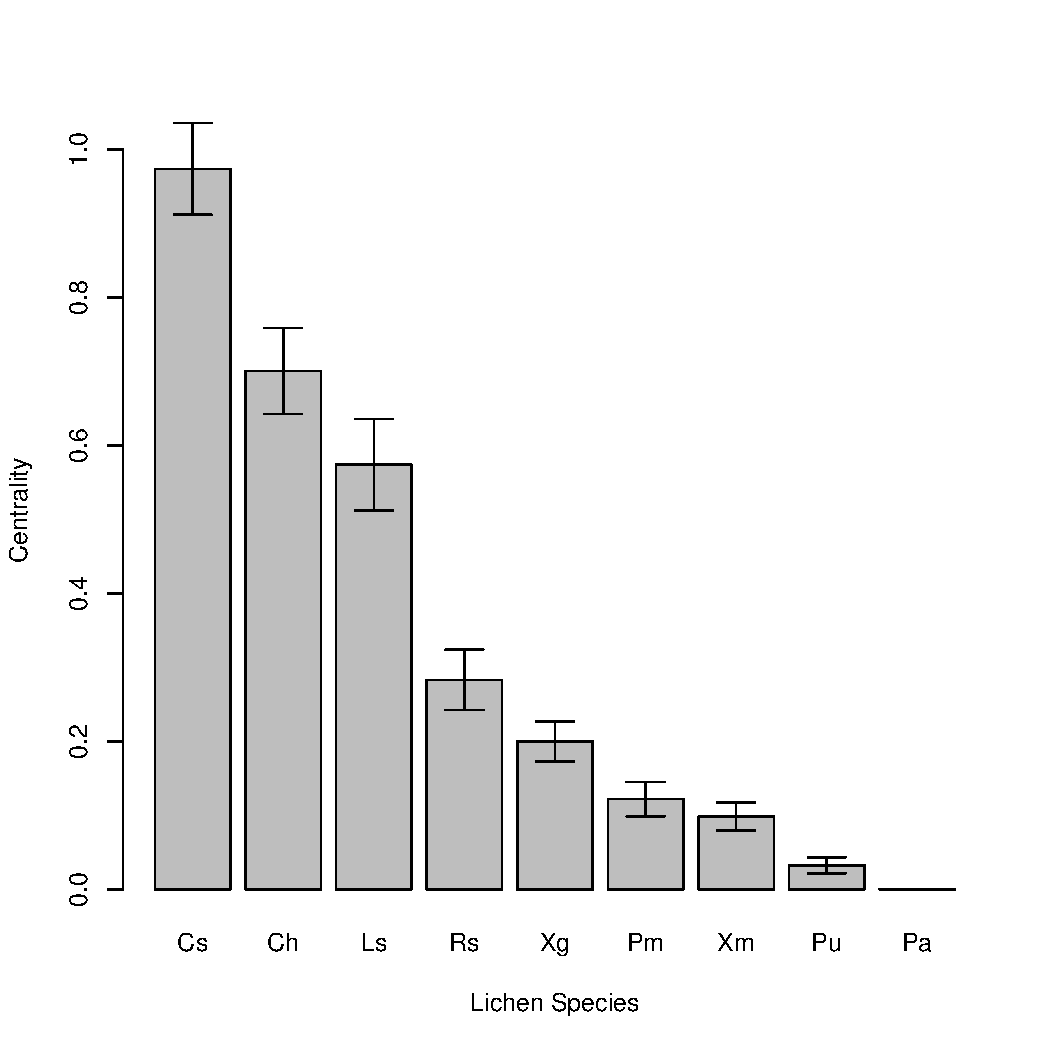
\includegraphics[width=\linewidth]{figures/spp_cen.pdf}
\caption{The relative centrality varied among the species of lichen
  observed in the common garden. Barplot showing the mean centrality
  ($\pm$ 1 S.E.) of the lichen species averaged across all trees that
  were observed.}
\label{fig:spp_cen}
\end{figure}

\end{document}
